% answers.tex —— 2020 年·江苏卷 · 参考答案与详细解析片段
% 由 tools/generate_projects.py 依来源总账自 2020/2020_数学真题_江苏_试题.md + 2020/2020_数学真题_江苏_解析正文.md + 2020/2020_数学真题_江苏_答案要点.md 生成，勿手改（改源 MD 后重跑）


\begin{answer}
\gksolhead{1}{}

\textbf{题目}：

已知集合 $A=\{-1,0,1,2\}$，$B=\{0,2,3\}$，则 $A\cap B=$\gkblank{}。

\Needspace{4\baselineskip}
\textbf{解析}

\Needspace{5\baselineskip}
$A=\{-1,0,1,2\}$，$B=\{0,2,3\}$，逐个比较两集合的元素：$-1\notin B$，$1\notin B$，$3\notin A$，只有 $0$ 与 $2$ 同时属于两个集合。故
\nopagebreak[4]
\[A\cap B=\{0,2\}.\]

\gkanswer{答案：$\{0,2\}$。$A$ 与 $B$ 的公共元素只有 $0$ 与 $2$。}

\end{answer}
\begin{answer}
\gksolhead{2}{}

\textbf{题目}：

已知 $\mathrm i$ 是虚数单位，则复数 $z=(1+\mathrm i)(2-\mathrm i)$ 的实部是\gkblank{}。

\Needspace{4\baselineskip}
\textbf{解析}

\Needspace{5\baselineskip}
按多项式乘法展开，并注意 $\mathrm i^2=-1$：
\nopagebreak[4]
\[z=(1+\mathrm i)(2-\mathrm i)=2-\mathrm i+2\mathrm i-\mathrm i^2=2+\mathrm i+1=3+\mathrm i .\]
所以 $z$ 的实部为 $3$。

\gkanswer{答案：$3$。$z=(1+\mathrm i)(2-\mathrm i)=2-\mathrm i+2\mathrm i-\mathrm i^2=3+\mathrm i$，实部为 $3$。}

\end{answer}
\begin{answer}
\gksolhead{3}{}

\textbf{题目}：

已知一组数据 $4,2a,3-a,5,6$ 的平均数为 $4$，则 $a$ 的值是\gkblank{}。

\Needspace{4\baselineskip}
\textbf{解析}

\Needspace{5\baselineskip}
五个数据的平均数为 $4$，故总和为 $5\times4=20$：
\nopagebreak[4]
\[4+2a+(3-a)+5+6=20\ \Longrightarrow\ 18+a=20\ \Longrightarrow\ a=2 .\]
回代检验：数据为 $4,4,1,5,6$，和为 $20$，平均数为 $4$ 。

\gkanswer{答案：$2$。由 $\dfrac{4+2a+3-a+5+6}5=4$ 得 $18+a=20$，故 $a=2$。}

\end{answer}
\begin{answer}
\gksolhead{4}{}

\textbf{题目}：

将一颗质地均匀的正方体骰子先后抛掷 $2$ 次，观察向上的点数，则点数和为 $5$ 的概率是\gkblank{}。

\Needspace{4\baselineskip}
\textbf{解析}

\Needspace{5\baselineskip}
先后抛掷两次共有 $6\times6=36$ 个等可能结果。点数和为 $5$ 的情形只有
\nopagebreak[4]
\[(1,4),\ (2,3),\ (3,2),\ (4,1),\]
\Needspace{5\baselineskip}
共 $4$ 个。故所求概率为
\nopagebreak[4]
\[P=\frac4{36}=\frac19 .\]

\gkanswer{答案：$\dfrac19$。点数和为 $5$ 的有 $(1,4),(2,3),(3,2),(4,1)$ 共 $4$ 种，概率为 $\dfrac4{36}=\dfrac19$。}

\end{answer}
\begin{answer}
\gksolhead{5}{}

\textbf{题目}：

如图是一个算法流程图。若输出 $y$ 的值为 $-2$，则输入 $x$ 的值是\gkblank{}。
\nopagebreak[4]
\begin{center}% 2020 江苏卷 5：算法流程图（开始→输入 x→判断 x>0→是 y←2^x / 否 y←x+1→输出 y→结束）
% 绘制依据：固定源 PDF 第 1115 面原图。原图自上而下的主干与左「Y」右「N」的分支走向照录。
\begin{tikzpicture}[scale=0.92, font=\small, >=Stealth,
    box/.style={draw, minimum width=2.0cm, minimum height=0.72cm, align=center},
    io/.style={draw, trapezium, trapezium left angle=72, trapezium right angle=108,
      minimum width=2.2cm, minimum height=0.72cm, align=center},
    dec/.style={draw, diamond, aspect=2.1, inner sep=1pt, align=center}]
  \node[draw, rounded corners=6pt, minimum width=1.7cm, minimum height=0.72cm] (begin) at (0,0) {开始};
  \node[io] (in) at (0,-1.35) {输入 $x$};
  \node[dec] (judge) at (0,-2.85) {$x>0$?};
  \node[box] (yes) at (-2.5,-4.4) {$y\leftarrow 2^{x}$};
  \node[box] (no) at (2.5,-4.4) {$y\leftarrow x+1$};
  \node[io] (out) at (0,-5.85) {输出 $y$};
  \node[draw, rounded corners=6pt, minimum width=1.7cm, minimum height=0.72cm] (end) at (0,-7.15) {结束};

  \draw[->] (begin) -- (in);
  \draw[->] (in) -- (judge);
  \draw[->] (judge.west) -| (yes.north);
  \node at (-1.85,-2.55) {$Y$};
  \draw[->] (judge.east) -| (no.north);
  \node at (1.85,-2.55) {$N$};
  \draw[->] (yes.south) |- (out.west);
  \draw[->] (no.south) |- (out.east);
  \draw[->] (out) -- (end);
\end{tikzpicture}
\end{center}
\nopagebreak[4]
\Needspace{4\baselineskip}
\textbf{解析}

流程图的分支为：$x>0$ 时 $y=2^x$；$x\leqslant0$ 时 $y=x+1$。

\Needspace{5\baselineskip}
若 $x>0$，则 $y=2^x>0$，不可能等于 $-2$，故只能走 $x\leqslant0$ 的分支：
\nopagebreak[4]
\[x+1=-2\ \Longrightarrow\ x=-3 .\]
检验：$x=-3\leqslant0$，走 $y=x+1$ 分支，$y=-2$ 。

\gkanswer{答案：$-3$。$x>0$ 时 $y=2^x>0$，不可能等于 $-2$；故 $x\leqslant0$，由 $x+1=-2$ 得 $x=-3$。}

\end{answer}
\begin{answer}
\gksolhead{6}{}

\textbf{题目}：

在平面直角坐标系 $xOy$ 中，若双曲线 $\dfrac{x^2}{a^2}-\dfrac{y^2}{5}=1$（$a>0$）的一条渐近线方程为 $y=\dfrac{\sqrt5}{2}x$，则该双曲线的离心率是\gkblank{}。

\Needspace{4\baselineskip}
\textbf{解析}

\Needspace{5\baselineskip}
双曲线 $\dfrac{x^2}{a^2}-\dfrac{y^2}{b^2}=1$ 的渐近线为 $y=\pm\dfrac bax$。本题 $b^2=5$，即 $b=\sqrt5$，由题设的一条渐近线 $y=\dfrac{\sqrt5}2x$ 得
\nopagebreak[4]
\[\frac ba=\frac{\sqrt5}{2}\ \Longrightarrow\ \frac{\sqrt5}{a}=\frac{\sqrt5}{2}\ \Longrightarrow\ a=2 .\]
\Needspace{5\baselineskip}
于是 $c=\sqrt{a^2+b^2}=\sqrt{4+5}=3$，离心率
\nopagebreak[4]
\[e=\frac ca=\frac32 .\]

\gkanswer{答案：$\dfrac32$。由 $\dfrac{b}{a}=\dfrac{\sqrt5}{2}$ 且 $b^2=5$ 得 $a=2$、$c=\sqrt{a^2+b^2}=3$，故 $e=\dfrac ca=\dfrac32$。}

\end{answer}
\begin{answer}
\gksolhead{7}{}

\textbf{题目}：

已知 $y=f(x)$ 是奇函数，当 $x\geqslant0$ 时，$f(x)=x^{\frac23}$，则 $f(-8)$ 的值是\gkblank{}。

\Needspace{4\baselineskip}
\textbf{解析}

\Needspace{5\baselineskip}
$f(x)$ 是奇函数，故 $f(-8)=-f(8)$。又 $8\geqslant0$，用给定表达式：
\nopagebreak[4]
\[f(8)=8^{\frac23}=\left(2^3\right)^{\frac23}=2^2=4 .\]
\Needspace{5\baselineskip}
所以
\nopagebreak[4]
\[f(-8)=-4 .\]

\gkanswer{答案：$-4$。$f(-8)=-f(8)=-8^{\frac23}=-4$。}

\end{answer}
\begin{answer}
\gksolhead{8}{}

\textbf{题目}：

已知 $\sin^2\left(\dfrac\pi4+\alpha\right)=\dfrac23$，则 $\sin2\alpha$ 的值是\gkblank{}。

\Needspace{4\baselineskip}
\textbf{解析}

\Needspace{5\baselineskip}
用降幂公式把平方化成一次式。由 $\cos2\theta=1-2\sin^2\theta$ 得
\nopagebreak[4]
\[\sin^2\left(\frac\pi4+\alpha\right)=\frac{1-\cos\left(\frac\pi2+2\alpha\right)}2 .\]
\Needspace{5\baselineskip}
又 $\cos\left(\dfrac\pi2+2\alpha\right)=-\sin2\alpha$，故
\nopagebreak[4]
\[\frac{1+\sin2\alpha}{2}=\frac23\ \Longrightarrow\ \sin2\alpha=\frac43-1=\frac13 .\]

\gkanswer{答案：$\dfrac13$。由 $\sin^2\left(\dfrac\pi4+\alpha\right)=\dfrac{1+\sin2\alpha}2=\dfrac23$ 得 $\sin2\alpha=\dfrac13$。}

\end{answer}
\begin{answer}
\gksolhead{9}{}

\textbf{题目}：

如图，六角螺帽毛坯是由一个正六棱柱挖去一个圆柱所构成的。已知螺帽的底面正六边形边长为 $2\ \mathrm{cm}$，高为 $2\ \mathrm{cm}$，内孔半径为 $0.5\ \mathrm{cm}$，则此六角螺帽毛坯的体积是\gkblank{}$\mathrm{cm}^2$。
\nopagebreak[4]
\begin{center}% 2020 江苏卷 9：六角螺帽毛坯（正六棱柱挖去一个圆柱）
% 绘制依据：固定源 PDF 第 1115 面原图。正六棱柱竖放，顶面为压扁的正六边形（前后各一条水平边），
% 顶面中心为一个圆柱形内孔（椭圆口），孔壁用虚线画到底面的虚线椭圆；背面棱与底面的后侧棱为虚线。
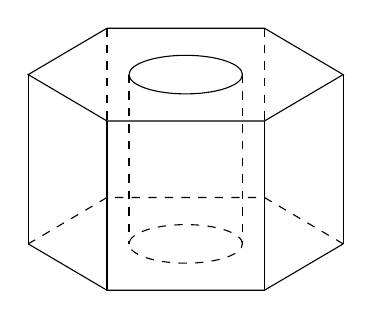
\begin{tikzpicture}[scale=1.0, font=\small]
  \def\r{2}
  \def\sq{0.34}
  \def\hh{2.15}
  % 顶面六顶点（角度 0,60,...,300），y 方向压缩为 \sq 倍
  \coordinate (P0) at ({\r*cos(0)},{\sq*\r*sin(0)});
  \coordinate (P1) at ({\r*cos(60)},{\sq*\r*sin(60)});
  \coordinate (P2) at ({\r*cos(120)},{\sq*\r*sin(120)});
  \coordinate (P3) at ({\r*cos(180)},{\sq*\r*sin(180)});
  \coordinate (P4) at ({\r*cos(240)},{\sq*\r*sin(240)});
  \coordinate (P5) at ({\r*cos(300)},{\sq*\r*sin(300)});
  % 底面六顶点：整体下移 \hh
  \coordinate (Q0) at ({\r*cos(0)},{\sq*\r*sin(0)-\hh});
  \coordinate (Q1) at ({\r*cos(60)},{\sq*\r*sin(60)-\hh});
  \coordinate (Q2) at ({\r*cos(120)},{\sq*\r*sin(120)-\hh});
  \coordinate (Q3) at ({\r*cos(180)},{\sq*\r*sin(180)-\hh});
  \coordinate (Q4) at ({\r*cos(240)},{\sq*\r*sin(240)-\hh});
  \coordinate (Q5) at ({\r*cos(300)},{\sq*\r*sin(300)-\hh});

  % 顶面轮廓（全可见，实线）
  \draw (P0) -- (P1) -- (P2) -- (P3) -- (P4) -- (P5) -- cycle;

  % 竖直棱：前面与左右两侧可见（实线），背面两条为虚线
  \draw (P0) -- (Q0);
  \draw (P3) -- (Q3);
  \draw (P4) -- (Q4);
  \draw (P5) -- (Q5);
  \draw[dashed] (P1) -- (Q1);
  \draw[dashed] (P2) -- (Q2);

  % 底面轮廓：前侧三条边可见（实线），后侧三条边被遮挡（虚线）
  \draw (Q3) -- (Q4) -- (Q5) -- (Q0);
  \draw[dashed] (Q0) -- (Q1) -- (Q2) -- (Q3);

  % 内孔：顶面椭圆口（实线），孔沿两条竖直线（虚线），底面椭圆（虚线）
  \draw (0,0) ellipse (0.72 and 0.245);
  \draw[dashed] (-0.72,0) -- (-0.72,-\hh);
  \draw[dashed] (0.72,0) -- (0.72,-\hh);
  \draw[dashed] (0,-\hh) ellipse (0.72 and 0.245);
\end{tikzpicture}
\end{center}
\nopagebreak[4]
\Needspace{4\baselineskip}
\textbf{解析}

毛坯体积 = 正六棱柱体积 $-$ 圆柱形内孔体积。

\Needspace{5\baselineskip}
底面正六边形边长为 $2$，面积
\nopagebreak[4]
\[S=6\times\frac{\sqrt3}{4}\times2^2=6\sqrt3 .\]
\Needspace{5\baselineskip}
正六棱柱高为 $2$，体积 $V_1=6\sqrt3\times2=12\sqrt3$。内孔是底面半径 $0.5$、高 $2$ 的圆柱，体积
\nopagebreak[4]
\[V_2=\pi\times0.5^2\times2=\frac\pi2 .\]
\Needspace{5\baselineskip}
所以毛坯体积为
\nopagebreak[4]
\[V=V_1-V_2=12\sqrt3-\frac\pi2\ \left(\mathrm{cm}^3\right).\]
数值约 $19.21$。原页把单位印作 $\mathrm{cm}^2$，与「体积」不符，应为 $\mathrm{cm}^3$。

\gkanswer{答案：$12\sqrt3-\dfrac\pi2$。底面正六边形面积 $6\times\dfrac{\sqrt3}4\times2^2=6\sqrt3$，正六棱柱体积 $6\sqrt3\times2=12\sqrt3$，内孔圆柱体积 $\pi\times0.5^2\times2=\dfrac\pi2$，故体积为 $12\sqrt3-\dfrac\pi2$（$\mathrm{cm}^3$）。}

\end{answer}
\begin{answer}
\gksolhead{10}{}

\textbf{题目}：

将函数 $y=3\sin\left(2x+\dfrac\pi4\right)$ 的图象向右平移 $\dfrac\pi6$ 个单位长度，则平移后的图象中与 $y$ 轴最近的对称轴的方程是\gkblank{}。

\Needspace{4\baselineskip}
\textbf{解析}

\Needspace{5\baselineskip}
图象向右平移 $\dfrac\pi6$ 个单位，即把 $x$ 换成 $x-\dfrac\pi6$：
\nopagebreak[4]
\[y=3\sin\left[2\left(x-\frac\pi6\right)+\frac\pi4\right]=3\sin\left(2x-\frac\pi3+\frac\pi4\right)=3\sin\left(2x-\frac{\pi}{12}\right).\]
\Needspace{5\baselineskip}
对称轴满足 $2x-\dfrac\pi{12}=\dfrac\pi2+k\pi$，即
\nopagebreak[4]
\[x=\frac{7\pi}{24}+\frac{k\pi}{2}\quad(k\in\mathbf Z).\]
\Needspace{5\baselineskip}
取 $k=0$ 得 $x=\dfrac{7\pi}{24}$；取 $k=-1$ 得 $x=\dfrac{7\pi}{24}-\dfrac\pi2=-\dfrac{5\pi}{24}$。比较绝对值
\nopagebreak[4]
\[\left|-\frac{5\pi}{24}\right|=\frac{5\pi}{24}<\frac{7\pi}{24},\]
故与 $y$ 轴最近的对称轴是 $x=-\dfrac{5\pi}{24}$。

\gkanswer{答案：$x=-\dfrac{5\pi}{24}$。平移后 $y=3\sin\left(2x-\dfrac\pi{12}\right)$，对称轴 $x=\dfrac{7\pi}{24}+\dfrac{k\pi}2$，$k=0$ 与 $k=-1$ 中离 $y$ 轴最近的是 $-\dfrac{5\pi}{24}$。}

\end{answer}
\begin{answer}
\gksolhead{11}{}

\textbf{题目}：

设 $\{a_n\}$ 是公差为 $d$ 的等差数列，$\{b_n\}$ 是公比为 $q$ 的等比数列。已知数列 $\{a_n+b_n\}$ 的前 $n$ 项和 $S_n=n^2-n+2^n-1$（$n\in\mathbf N^*$），则 $d+q$ 的值是\gkblank{}。

\Needspace{4\baselineskip}
\textbf{解析}

\Needspace{5\baselineskip}
记 $S_0=0$，则 $a_n+b_n=S_n-S_{n-1}$（$n\geqslant1$）。当 $n\geqslant2$ 时
\nopagebreak[4]
\[a_n+b_n=\left(n^2-n+2^n-1\right)-\left[(n-1)^2-(n-1)+2^{n-1}-1\right]=2n-2+2^{n-1}.\]
\Needspace{5\baselineskip}
$n=1$ 时右式为 $0+1=1$，而 $a_1+b_1=S_1=1-1+2-1=1$，故对一切 $n\geqslant1$ 有
\nopagebreak[4]
\[a_n+b_n=2n-2+2^{n-1}.\]

\Needspace{5\baselineskip}
设 $a_n=a_1+(n-1)d$，$b_n=b_1q^{n-1}$。等式两边的指数项须对一切 $n$ 恒等：
\nopagebreak[4]
\[b_1q^{n-1}=2^{n-1}\ \Longrightarrow\ q=2,\ b_1=1 .\]
（若 $q=1$，左端为常数，不可能等于 $2^{n-1}$。）剩下的线性部分给出 $a_n=2n-2$，即 $a_1=0$，$d=2$。

\Needspace{5\baselineskip}
所以
\nopagebreak[4]
\[d+q=2+2=4 .\]

\gkanswer{答案：$4$。由 $a_n+b_n=S_n-S_{n-1}=2n-2+2^{n-1}$（$n\geqslant1$，$S_0=0$）得 $d=2$、$q=2$，故 $d+q=4$。}

\end{answer}
\begin{answer}
\gksolhead{12}{}

\textbf{题目}：

已知 $5x^2y^2+y^4=1$（$x,y\in\mathbf R$），则 $x^2+y^2$ 的最小值是\gkblank{}。

\Needspace{4\baselineskip}
\textbf{解析}

\Needspace{5\baselineskip}
令 $v=y^2$，则 $v\geqslant0$。由 $5x^2y^2+y^4=1$ 得 $v^2+5x^2v=1$，即
\nopagebreak[4]
\[x^2=\frac{1-v^2}{5v}.\]
\Needspace{5\baselineskip}
因为 $x^2\geqslant0$ 且 $v>0$，所以 $0<v\leqslant1$。于是
\nopagebreak[4]
\[x^2+y^2=\frac{1-v^2}{5v}+v=\frac{1+4v^2}{5v}=\frac1{5v}+\frac{4v}{5}.\]
\Needspace{5\baselineskip}
由均值不等式
\nopagebreak[4]
\[\frac1{5v}+\frac{4v}{5}\geqslant2\sqrt{\frac1{5v}\cdot\frac{4v}{5}}=2\sqrt{\frac4{25}}=\frac45,\]
等号当 $\dfrac1{5v}=\dfrac{4v}5$，即 $v^2=\dfrac14$、$v=\dfrac12$ 时成立（此时 $x^2=\dfrac3{10}$，检验 $5\cdot\dfrac3{10}\cdot\dfrac12+\dfrac14=\dfrac34+\dfrac14=1$ ）。

故最小值为 $\dfrac45$。

\gkanswer{答案：$\dfrac45$。令 $v=y^2\in(0,1]$，则 $x^2=\dfrac{1-v^2}{5v}$，$x^2+y^2=\dfrac1{5v}+\dfrac{4v}5\geqslant2\sqrt{\dfrac4{25}}=\dfrac45$，$v=\dfrac12$ 时取到。}

\end{answer}
\begin{answer}
\gksolhead{13}{}

\textbf{题目}：

在 $\triangle ABC$ 中，$AB=4$，$AC=3$，$\angle BAC=90^\circ$，$D$ 在边 $BC$ 上，延长 $AD$ 到 $P$，使得 $AP=9$。若 $\overrightarrow{PA}=m\overrightarrow{PB}+\left(\dfrac32-m\right)\overrightarrow{PC}$（$m$ 为常数），则 $CD$ 的长度是\gkblank{}。
\nopagebreak[4]
\begin{center}% 2020 江苏卷 13：△ABC 中 D 在边 BC 上，延长 AD 到 P（AP=9）
% 绘制依据：固定源 PDF 第 1115 面原图。A 左下、B 右下、C 左上（∠BAC=90°），
% D 在 BC 上，连 PA、PB、PC（P 在右方远处）。只标 A、B、C、D、P 五点。
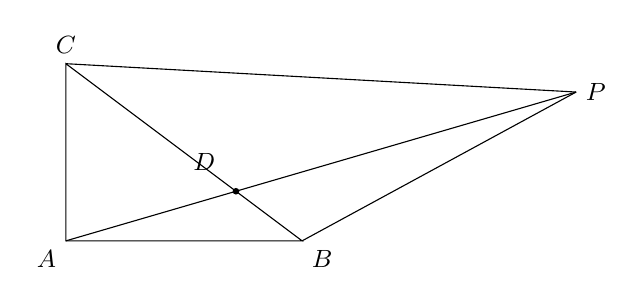
\begin{tikzpicture}[scale=0.75, font=\small]
  \coordinate (A) at (0,0);
  \coordinate (B) at (4,0);
  \coordinate (C) at (0,3);
  \coordinate (D) at (2.88,0.84);
  \coordinate (P) at (8.64,2.52);
  \draw (A) -- (B) -- (C) -- cycle;
  \draw (A) -- (P);
  \draw (B) -- (P);
  \draw (C) -- (P);
  \fill (D) circle (1.6pt);
  \node[below left] at (A) {$A$};
  \node[below right] at (B) {$B$};
  \node[above] at (C) {$C$};
  \node[above left=4pt] at (D) {$D$};
  \node[right] at (P) {$P$};
\end{tikzpicture}
\end{center}
\nopagebreak[4]
\Needspace{4\baselineskip}
\textbf{解析}

\Needspace{5\baselineskip}
以 $A$ 为原点、$AB$ 为 $x$ 轴正方向、$AC$ 为 $y$ 轴正方向建系：
\nopagebreak[4]
\[A(0,0),\quad B(4,0),\quad C(0,3).\]
\Needspace{5\baselineskip}
设 $P$ 的坐标向量为 $\boldsymbol p$。由 $\overrightarrow{PA}=m\overrightarrow{PB}+\left(\dfrac32-m\right)\overrightarrow{PC}$ 得
\nopagebreak[4]
\[-\boldsymbol p=m\left[(4,0)-\boldsymbol p\right]+\left(\frac32-m\right)\left[(0,3)-\boldsymbol p\right],\]
\Needspace{5\baselineskip}
即
\nopagebreak[4]
\[-\boldsymbol p=m(4,0)+\left(\frac32-m\right)(0,3)-\frac32\boldsymbol p .\]
\Needspace{5\baselineskip}
移项得 $\dfrac12\boldsymbol p=\left(4m,\ \dfrac92-3m\right)$，故
\nopagebreak[4]
\[\boldsymbol p=(8m,\ 9-6m).\]
\Needspace{5\baselineskip}
由 $AP=9$：
\nopagebreak[4]
\[64m^2+(9-6m)^2=81\ \Longrightarrow\ 100m^2-108m=0\ \Longrightarrow\ m=0\ \text{\text{或}}\ m=\frac{27}{25}.\]

\Needspace{5\baselineskip}
$m=0$ 时 $\boldsymbol p=(0,9)$，$P$ 落在射线 $AC$ 上，$AD$ 与 $AC$ 重合，$D$ 只能是 $C$，与「$D$ 在边 $BC$ 上、延长 $AD$ 到 $P$」的图形不符（此时 $CD=0$），故舍去。取 $m=\dfrac{27}{25}$，得
\nopagebreak[4]
\[P\left(\frac{216}{25},\frac{63}{25}\right).\]

\Needspace{5\baselineskip}
$D$ 在射线 $AP$ 上且在直线 $BC:x\cdot\dfrac14+y\cdot\dfrac13=1$ 上，设 $D=\lambda\boldsymbol p$，则
\nopagebreak[4]
\[\lambda\left(\frac{216}{25\cdot4}+\frac{63}{25\cdot3}\right)=1\ \Longrightarrow\ \lambda\left(\frac{54}{25}+\frac{21}{25}\right)=1\ \Longrightarrow\ \lambda=\frac13 .\]
\Needspace{5\baselineskip}
所以 $AD=\dfrac13AP=3$，$D\left(\dfrac{72}{25},\dfrac{21}{25}\right)$。于是
\nopagebreak[4]
\[CD=\sqrt{\left(\frac{72}{25}\right)^2+\left(\frac{21}{25}-3\right)^2}=\frac{\sqrt{72^2+54^2}}{25}=\frac{90}{25}=\frac{18}{5}.\]
另法检验：$BC=5$，$BD=\sqrt{\left(4-\frac{72}{25}\right)^2+\left(\frac{21}{25}\right)^2}=\frac{35}{25}=\frac75$，故 $CD=5-\dfrac75=\dfrac{18}5$ 。

\gkanswer{答案：$\dfrac{18}5$。由 $\overrightarrow{PA}=m\overrightarrow{PB}+\left(\dfrac32-m\right)\overrightarrow{PC}$ 与 $|\overrightarrow{PA}|=9$ 解得 $m=\dfrac{27}{25}$，此时 $AD=3$、$BD=\dfrac75$，故 $CD=5-\dfrac75=\dfrac{18}5$。}

\end{answer}
\begin{answer}
\gksolhead{14}{}

\textbf{题目}：

在平面直角坐标系 $xOy$ 中，已知 $P\left(\dfrac{\sqrt3}2,0\right)$，$A$，$B$ 是圆 $C:x^2+\left(y-\dfrac12\right)^2=36$ 上的两个动点，满足 $PA=PB$，则 $\triangle PAB$ 面积的最大值是\gkblank{}。

\Needspace{4\baselineskip}
\textbf{解析}

\Needspace{5\baselineskip}
圆心 $C_0\left(0,\dfrac12\right)$，半径 $6$，而
\nopagebreak[4]
\[|PC_0|=\sqrt{\left(\frac{\sqrt3}2\right)^2+\left(\frac12\right)^2}=1 .\]
$PA=PB$ 说明 $P$ 在弦 $AB$ 的垂直平分线上，而弦的垂直平分线必过圆心，故 $AB\perp PC_0$，且 $AB$ 被直线 $PC_0$ 垂直平分。

\Needspace{5\baselineskip}
设圆心 $C_0$ 到直线 $AB$ 的距离为 $d$（$0\leqslant d\leqslant6$），则
\nopagebreak[4]
\[|AB|=2\sqrt{36-d^2}.\]
\Needspace{5\baselineskip}
直线 $AB$ 有两条（关于 $C_0$ 对称），$P$ 到 $AB$ 的距离分别为 $|d-1|$ 与 $d+1$；取较大者 $d+1$，得
\nopagebreak[4]
\[S(d)=\frac12\cdot2\sqrt{36-d^2}\cdot(d+1)=\sqrt{36-d^2}\,(d+1).\]
\Needspace{5\baselineskip}
求导：
\nopagebreak[4]
\[S'(d)=\sqrt{36-d^2}-\frac{d(d+1)}{\sqrt{36-d^2}}=\frac{36-d-2d^2}{\sqrt{36-d^2}},\]
\Needspace{5\baselineskip}
令 $S'(d)=0$ 得 $2d^2+d-36=0$，即 $d=4$（另一根 $d=-\dfrac92$ 舍去）。比较
\nopagebreak[4]
\[S(4)=\sqrt{20}\times5=10\sqrt5,\qquad S(0)=6,\qquad S(6)=0,\]
故面积的最大值为 $10\sqrt5$（此时 $|AB|=4\sqrt5$，$P$ 到 $AB$ 的距离为 $5$）。

\gkanswer{答案：$10\sqrt5$。$PA=PB$ 使 $AB\perp PC$ 且被 $PC$ 垂直平分，设圆心到 $AB$ 的距离为 $d$，则面积 $S=\sqrt{36-d^2}\,(d+1)$，$d=4$ 时取最大值 $10\sqrt5$。}

\end{answer}
\begin{answer}
\gksolhead{15}{}

\textbf{题目}：

在三棱柱 $ABC-A_1B_1C_1$ 中，$AB\perp AC$，$B_1C\perp$ 平面 $ABC$，$E$，$F$ 分别是 $AC$，$B_1C$ 的中点。

（1） 求证：$EF\parallel$ 平面 $AB_1C_1$；

（2） 求证：平面 $AB_1C\perp$ 平面 $ABB_1$。
\nopagebreak[4]
\begin{center}% 2020 江苏卷 15：三棱柱 ABC-A1B1C1，E、F 分别为 AC、B1C 的中点
% 绘制依据：固定源 PDF 第 1115 面原图。斜置三棱柱：底面三角形 A 左、B 前下、C 右，
% A1、B1、C1 分别位于 A、B、C 的正上偏右（同一平移向量）。可见棱实线，隐蔽棱虚线。
% 图中另画出 AB1（实线）与 AC1（虚线，体内对角线），E 在 AC 上、F 在 B1C 上。
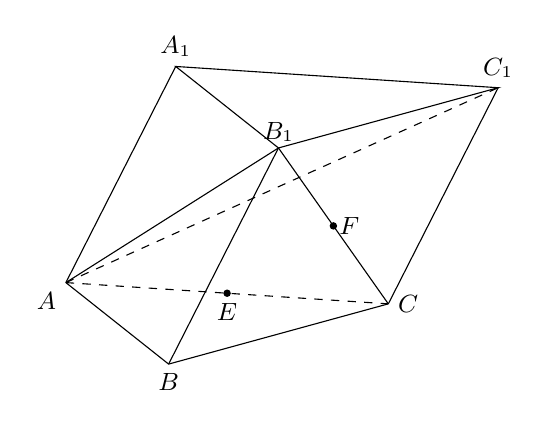
\begin{tikzpicture}[scale=0.9, font=\small]
  \coordinate (A) at (0,0);
  \coordinate (B) at (1.45,-1.15);
  \coordinate (C) at (4.55,-0.30);
  \coordinate (A1) at (1.55,3.05);
  \coordinate (B1) at (3.00,1.90);
  \coordinate (C1) at (6.10,2.75);
  \coordinate (E) at (2.275,-0.15);
  \coordinate (F) at (3.775,0.80);

  % 底面三角形
  \draw (A) -- (B) -- (C);
  \draw[dashed] (A) -- (C);
  % 侧棱
  \draw (A) -- (A1);
  \draw (B) -- (B1);
  \draw (C) -- (C1);
  % 顶面三角形
  \draw (A1) -- (B1) -- (C1) -- cycle;
  % 题设涉及的线段：AB1 实线，AC1 体内对角线（虚线），B1C 实线
  \draw (A) -- (B1);
  \draw[dashed] (A) -- (C1);
  \draw (B1) -- (C);

  \fill (E) circle (1.5pt);
  \fill (F) circle (1.5pt);
  \node[below left] at (A) {$A$};
  \node[below] at (B) {$B$};
  \node[right] at (C) {$C$};
  \node[above] at (A1) {$A_1$};
  \node[above, inner sep=2pt] at (B1) {$B_1$};
  \node[above] at (C1) {$C_1$};
  \node[below=2pt, inner sep=1.5pt] at (E) {$E$};
  \node[right, inner sep=2pt] at (F) {$F$};
\end{tikzpicture}
\end{center}
\nopagebreak[4]
\Needspace{4\baselineskip}
\textbf{解析}

\gksubpart{（1）}

\Needspace{5\baselineskip}
在 $\triangle AB_1C$ 中，$E$ 是 $AC$ 的中点，$F$ 是 $B_1C$ 的中点，由三角形中位线定理
\nopagebreak[4]
\[EF\parallel AB_1 .\]
\Needspace{5\baselineskip}
又 $AB_1\subset$ 平面 $AB_1C_1$，而 $EF\not\subset$ 平面 $AB_1C_1$（$E$ 在 $AC$ 上，$AC$ 与平面 $AB_1C_1$ 只交于 $A$，$E\neq A$），由线面平行的判定定理得
\nopagebreak[4]
\[EF\parallel\text{\text{平面} }AB_1C_1 .\]

\gksubpart{（2）}

\Needspace{5\baselineskip}
由 $B_1C\perp$ 平面 $ABC$，而 $AB\subset$ 平面 $ABC$，得
\nopagebreak[4]
\[B_1C\perp AB .\]
\Needspace{5\baselineskip}
又已知 $AB\perp AC$，且 $AC$ 与 $B_1C$ 是平面 $AB_1C$ 内两条相交直线（交于 $C$），故
\nopagebreak[4]
\[AB\perp\text{\text{平面} }AB_1C .\]
\Needspace{5\baselineskip}
而 $AB\subset$ 平面 $ABB_1$，由面面垂直的判定定理得
\nopagebreak[4]
\[\text{\text{平面} }AB_1C\perp\text{\text{平面} }ABB_1 .\]

\gkanswer{答案（1）：证明。$E$，$F$ 分别是 $AC$，$B_1C$ 的中点，故 $EF\parallel AB_1$；又 $AB_1\subset$ 平面 $AB_1C_1$ 而 $EF\not\subset$ 平面 $AB_1C_1$，所以 $EF\parallel$ 平面 $AB_1C_1$。}

\gkanswer{答案（2）：证明。$B_1C\perp$ 平面 $ABC$ 给出 $B_1C\perp AB$，又 $AB\perp AC$，故 $AB\perp$ 平面 $AB_1C$；而 $AB\subset$ 平面 $ABB_1$，所以平面 $AB_1C\perp$ 平面 $ABB_1$。}

\end{answer}
\begin{answer}
\gksolhead{16}{}

\textbf{题目}：

在 $\triangle ABC$ 中，角 $A,B,C$ 的对边分别为 $a,b,c$，已知 $a=3$，$c=\sqrt2$，$B=45^\circ$。

（1） 求 $\sin C$ 的值；

（2） 在边 $BC$ 上取一点 $D$，使得 $\cos\angle ADC=-\dfrac45$，求 $\tan\angle DAC$ 的值。
\nopagebreak[4]
\begin{center}% 2020 江苏卷 16：△ABC 中 D 在边 BC 上
% 绘制依据：固定源 PDF 第 1115 面原图。A 在上方偏右，B 左下、C 右下，D 在 BC 上靠近 C，
% 连 AD。只标 A、B、C、D 四点。
\begin{tikzpicture}[scale=1.05, font=\small]
  \coordinate (A) at (2.55,1.85);
  \coordinate (B) at (0,0);
  \coordinate (C) at (5.0,0);
  \coordinate (D) at (3.75,0);
  \draw (A) -- (B) -- (C) -- cycle;
  \draw (A) -- (D);
  \node[above] at (A) {$A$};
  \node[below left] at (B) {$B$};
  \node[below right] at (C) {$C$};
  \node[below=5pt, inner sep=3pt] at (D) {$D$};
\end{tikzpicture}
\end{center}
\nopagebreak[4]
\Needspace{4\baselineskip}
\textbf{解析}

\gksubpart{（1）}

\Needspace{5\baselineskip}
由余弦定理
\nopagebreak[4]
\[b^2=a^2+c^2-2ac\cos B=9+2-2\times3\times\sqrt2\times\frac{\sqrt2}2=11-6=5,\]
\Needspace{5\baselineskip}
故 $b=\sqrt5$。再由正弦定理 $\dfrac{b}{\sin B}=\dfrac{c}{\sin C}$ 得
\nopagebreak[4]
\[\sin C=\frac{c\sin B}{b}=\frac{\sqrt2\times\frac{\sqrt2}2}{\sqrt5}=\frac1{\sqrt5}=\frac{\sqrt5}5 .\]

\gksubpart{（2）}

\Needspace{5\baselineskip}
由 $\cos\angle ADC=-\dfrac45<0$ 知 $\angle ADC$ 为钝角，故
\nopagebreak[4]
\[\sin\angle ADC=\frac35,\qquad \tan\angle ADC=\frac{\sin\angle ADC}{\cos\angle ADC}=-\frac34 .\]
又 $c=\sqrt2<b=\sqrt5$，故 $C<B=45^\circ$，$C$ 为锐角，由 $\sin C=\dfrac1{\sqrt5}$ 得 $\cos C=\dfrac2{\sqrt5}$，于是 $\tan C=\dfrac12$。

\Needspace{5\baselineskip}
在 $\triangle ADC$ 中，
\nopagebreak[4]
\[\angle DAC=180^\circ-\angle ADC-C,\]
\Needspace{5\baselineskip}
所以
\nopagebreak[4]
\[\tan\angle DAC=-\tan\left(\angle ADC+C\right)=-\frac{\tan\angle ADC+\tan C}{1-\tan\angle ADC\cdot\tan C}
=-\frac{-\frac34+\frac12}{1+\frac38}=-\frac{-\frac14}{\frac{11}8}=\frac2{11}.\]

\gkanswer{答案（1）：$\dfrac{\sqrt5}5$。由余弦定理 $b^2=a^2+c^2-2ac\cos B=5$ 得 $b=\sqrt5$，再由正弦定理 $b\sin C=c\sin B$ 得 $\sin C=\dfrac{\sqrt5}5$。}

\gkanswer{答案（2）：$\dfrac2{11}$。$\sin\angle ADC=\dfrac35$，$\tan\angle ADC=-\dfrac34$，$\tan C=\dfrac12$，故 $\tan\angle DAC=\tan\left(180^\circ-\angle ADC-C\right)=\dfrac2{11}$。}

\end{answer}
\begin{answer}
\gksolhead{17}{}

\textbf{题目}：

某地准备在山谷中建一座桥梁，桥址位置的竖直截面图如图所示：谷底 $O$ 在水平线 $MN$ 上，桥 $AB$ 与 $MN$ 平行，$OO'$ 为铅垂线（$O'$ 在 $AB$ 上）。经测量，左侧曲线 $AO$ 上任一点 $D$ 到 $MN$ 的距离 $h_1$（米）与 $D$ 到 $OO'$ 的距离 $a$（米）之间满足关系式 $h_1=\dfrac1{40}a^2$；右侧曲线 $BO$ 上任一点 $F$ 到 $MN$ 的距离 $h_2$（米）与 $F$ 到 $OO'$ 的距离 $b$（米）之间满足关系式 $h_2=-\dfrac1{800}b^3+6b$。已知点 $B$ 到 $OO'$ 的距离为 $40$ 米。

（1） 求桥 $AB$ 的长度；

（2） 计划在谷底两侧建造平行于 $OO'$ 的桥墩 $CD$ 和 $EF$，且 $CE$ 为 $80$ 米，其中 $C$，$E$ 在 $AB$ 上（不包括端点）。桥墩 $EF$ 每米造价 $k$（万元）、桥墩 $CD$ 每米造价 $\dfrac32k$（万元）（$k>0$）。问 $O'E$ 为多少米时，桥墩 $CD$ 与 $EF$ 的总造价最低？
\nopagebreak[4]
\begin{center}% 2020 江苏卷 17：桥梁竖直截面（谷底 O 在水平线 MN 上，桥 AB∥MN，OO' 为铅垂线）
% 绘制依据：固定源 PDF 第 1115 面原图与题给关系式 h1=a^2/40、h2=-b^3/800+6b（B 到 OO' 为 40 米）。
% 坐标换算：横向 1 米 = 0.0475 单位，纵向 1 米 = 0.0225 单位；
% 左侧 a 自 O' 向左量（a=80 时 h1=160，即 A 点），右侧 b 自 O' 向右量（b=40 时 h2=160，即 B 点）。
% 图中标出 C、D、E、F、D1、O、F1 与 a、b、h1、h2；桥墩 CD、EF 为实线，各条量距线为虚线。
\begin{tikzpicture}[scale=1.0, font=\small]
  \def\ox{4.6}      % O' 的横坐标
  \def\ky{0.0225}   % 纵向比例（米 -> 单位）
  \def\kx{0.0475}   % 横向比例（米 -> 单位）
  \def\H{3.6}       % 桥面高 160 米

  % 水平线 MN
  \draw (-0.55,0) -- (8.3,0);
  \node[below] at (-0.45,0) {$M$};
  \node[below] at (8.2,0) {$N$};

  % 左曲线 h1=a^2/40（a 自 O' 向左量），绘到 A 点上方
  \draw[thick] plot[domain=0:92, samples=140]
    ({\ox-\kx*\x}, {\ky*\x*\x/40});
  % 右曲线 h2=-b^3/800+6b（b 自 O' 向右量），绘过 B 点后再下垂
  \draw[thick] plot[domain=0:46, samples=160]
    ({\ox+\kx*\x}, {\ky*(-0.00125*\x*\x*\x+6*\x)});

  % 桥面 AB（水平，与 MN 平行）
  \draw (0.80,\H) -- (6.50,\H);

  % 铅垂线 OO'
  \draw[dashed] (\ox,0) -- (\ox,\H);

  % 桥墩 CD：C 在桥面上，D 在左曲线（a=60 米）
  \draw (1.75,\H) -- (1.75,2.025);
  % 桥墩 EF：E 在桥面上，F 在右曲线（b=20 米）
  \draw (5.55,\H) -- (5.55,2.475);

  % D、F 到 MN 的虚线（h1、h2）
  \draw[dashed] (1.75,2.025) -- (1.75,0);
  \draw[dashed] (5.55,2.475) -- (5.55,0);
  % 量距 a、b 的虚线
  \draw[dashed] (1.75,2.025) -- (\ox,2.025);
  \draw[dashed] (5.55,2.475) -- (\ox,2.475);

  % 标注
  \node at (0.40,3.72) {$A$};
  \node[above] at (1.75,\H) {$C$};
  \node[above] at (\ox,\H) {$O'$};
  \node[above] at (5.55,\H) {$E$};
  \node at (6.62,3.80) {$B$};
  \node[left] at (1.72,2.03) {$D$};
  \node[right] at (5.58,2.44) {$F$};
  \node[below] at (1.75,0) {$D_1$};
  \node[below] at (\ox,0) {$O$};
  \node[below] at (5.55,0) {$F_1$};
  \node at (3.20,1.88) {$a$};
  \node at (5.02,2.70) {$b$};
  \node at (1.42,1.02) {$h_1$};
  \node at (5.92,1.42) {$h_2$};
\end{tikzpicture}
\end{center}
\nopagebreak[4]
\Needspace{4\baselineskip}
\textbf{解析}

\gksubpart{（1）}

\Needspace{5\baselineskip}
点 $B$ 到 $OO'$ 的距离为 $40$，即 $b=40$，故桥面高出 $MN$
\nopagebreak[4]
\[h_2(40)=-\frac{40^3}{800}+6\times40=-80+240=160\ (\text{\text{米}}).\]
\Needspace{5\baselineskip}
桥 $AB\parallel MN$，故 $A$ 的高度也是 $160$ 米。设 $A$ 到 $OO'$ 的距离为 $a$，由
\nopagebreak[4]
\[h_1(a)=\frac{a^2}{40}=160\ \Longrightarrow\ a^2=6400\ \Longrightarrow\ a=80 .\]
\Needspace{5\baselineskip}
所以
\nopagebreak[4]
\[AB=80+40=120\ (\text{\text{米}}).\]

\gksubpart{（2）}

\Needspace{5\baselineskip}
桥面到 $MN$ 的高为 $160$ 米，桥墩长度等于「桥面高」减去「墩底所在曲线点的高度」。设 $O'E=x$（米），则 $O'C=80-x$，由 $C$、$E$ 都在 $AB$ 上且不含端点得
\nopagebreak[4]
\[0<x<40 .\]

\Needspace{5\baselineskip}
于是
\nopagebreak[4]
\[EF=160-h_2(x)=160-\left(-\frac{x^3}{800}+6x\right)=160+\frac{x^3}{800}-6x,\]
\nopagebreak[4]
\[CD=160-h_1(80-x)=160-\frac{(80-x)^2}{40}.\]

\Needspace{5\baselineskip}
总造价（单位：万元）
\nopagebreak[4]
\[W(x)=k\cdot EF+\frac32k\cdot CD
=k\left[160+\frac{x^3}{800}-6x+\frac32\left(160-\frac{(80-x)^2}{40}\right)\right].\]
\Needspace{5\baselineskip}
化简括号内的式子：由 $\dfrac32\cdot\dfrac{(80-x)^2}{40}=\dfrac{3(80-x)^2}{80}=240-6x+\dfrac{3x^2}{80}$，得
\nopagebreak[4]
\[W(x)=k\left[160+\frac{x^3}{800}-6x+240-\left(240-6x+\frac{3x^2}{80}\right)\right]
=k\left[160+\frac{x^3}{800}-\frac{3x^2}{80}\right].\]
\Needspace{5\baselineskip}
求导：
\nopagebreak[4]
\[W'(x)=k\left(\frac{3x^2}{800}-\frac{6x}{80}\right)=\frac{3k}{800}x(x-20).\]
\Needspace{5\baselineskip}
当 $0<x<20$ 时 $W'(x)<0$，当 $20<x<40$ 时 $W'(x)>0$，故 $x=20$ 时 $W$ 取最小值
\nopagebreak[4]
\[W(20)=k\left(160+\frac{8000}{800}-\frac{3\times400}{80}\right)=k(160+10-15)=155k .\]
即 $O'E=20$ 米时总造价最低，最低总造价为 $155k$ 万元。

\gkanswer{答案（1）：$120$ 米。$B$ 处 $b=40$ 给出 $h_2=-\dfrac{40^3}{800}+240=160$；$A$ 处 $h_1=\dfrac{a^2}{40}=160$ 得 $a=80$，故 $AB=80+40=120$（米）。}

\gkanswer{答案（2）：$O'E=20$ 米时总造价最低，最低为 $155k$ 万元。设 $O'E=x$，则 $O'C=80-x$，$CD=160-\dfrac{(80-x)^2}{40}$，$EF=160-\left(-\dfrac{x^3}{800}+6x\right)$，总造价 $W(x)=k\left[\dfrac{x^3}{800}-\dfrac{3x^2}{80}+160\right]$，$W'(x)=\dfrac{3x(x-20)}{800}k$，故 $x=20$ 时取最小值。}

\end{answer}
\begin{answer}
\gksolhead{18}{}

\textbf{题目}：

在平面直角坐标系 $xOy$ 中，已知椭圆 $E:\dfrac{x^2}4+\dfrac{y^2}3=1$ 的左、右焦点分别为 $F_1$，$F_2$，点 $A$ 在椭圆 $E$ 上且在第一象限内，$AF_2\perp F_1F_2$，直线 $AF_1$ 与椭圆 $E$ 相交于另一点 $B$。

（1） 求 $\triangle AF_1F_2$ 的周长；

（2） 在 $x$ 轴上任取一点 $P$，直线 $AP$ 与椭圆 $E$ 的右准线相交于点 $Q$，求 $\overrightarrow{OP}\cdot\overrightarrow{QP}$ 的最小值；

（3） 设点 $M$ 在椭圆 $E$ 上，记 $\triangle OAB$ 与 $\triangle MAB$ 的面积分别为 $S_1$，$S_2$，若 $S_2=3S_1$，求点 $M$ 的坐标。

\Needspace{4\baselineskip}
\textbf{解析}

椭圆 $\dfrac{x^2}4+\dfrac{y^2}3=1$ 中 $a=2$，$b=\sqrt3$，$c=1$，故 $F_1(-1,0)$，$F_2(1,0)$，右准线为 $x=\dfrac{a^2}c=4$。

\gksubpart{（1）}

\Needspace{5\baselineskip}
$AF_2\perp F_1F_2$ 表明 $A$ 的横坐标为 $1$，代入椭圆得 $\dfrac14+\dfrac{y^2}3=1$，即 $y^2=\dfrac94$；$A$ 在第一象限，故 $A\left(1,\dfrac32\right)$。于是
\nopagebreak[4]
\[AF_2=\frac32,\qquad F_1F_2=2,\qquad AF_1=\sqrt{2^2+\left(\frac32\right)^2}=\frac52 .\]
\Needspace{5\baselineskip}
$\triangle AF_1F_2$ 的周长为
\nopagebreak[4]
\[\frac32+2+\frac52=6 .\]
（也可直接用 $AF_1+AF_2=2a=4$，周长 $=2a+2c=6$。）

\gksubpart{（2）}

\Needspace{5\baselineskip}
设 $P(p,0)$（$p\neq1$，否则 $AP$ 为竖直线，不与右准线相交）。直线 $AP$ 上的点可写成
\nopagebreak[4]
\[\left(1+t(p-1),\ \frac32(1-t)\right).\]
\Needspace{5\baselineskip}
令横坐标为 $4$，得 $1+t(p-1)=4$，即 $t=\dfrac3{p-1}$，于是
\nopagebreak[4]
\[Q\left(4,\ \frac32\left(1-\frac3{p-1}\right)\right)=\left(4,\ \frac{3(p-4)}{2(p-1)}\right).\]
\Needspace{5\baselineskip}
从而
\nopagebreak[4]
\[\overrightarrow{OP}=(p,0),\qquad \overrightarrow{QP}=\left(p-4,\ -\frac{3(p-4)}{2(p-1)}\right),\]
\nopagebreak[4]
\[\overrightarrow{OP}\cdot\overrightarrow{QP}=p(p-4)=(p-2)^2-4\geqslant-4 .\]
当 $p=2$ 时取到最小值 $-4$（此时 $Q(4,-3)$，检验：$\overrightarrow{OP}=(2,0)$，$\overrightarrow{QP}=(-2,3)$，点积为 $-4$ ）。

\gksubpart{（3）}

\Needspace{5\baselineskip}
先求 $B$。直线 $AF_1$ 过 $A\left(1,\dfrac32\right)$ 与 $F_1(-1,0)$，斜率为 $\dfrac34$，方程为 $y=\dfrac34(x+1)$。代入椭圆：
\nopagebreak[4]
\[\frac{x^2}4+\frac{1}{3}\cdot\frac{9}{16}(x+1)^2=1\ \Longrightarrow\ 4x^2+3(x+1)^2=16\ \Longrightarrow\ 7x^2+6x-13=0,\]
\Needspace{5\baselineskip}
即 $(7x+13)(x-1)=0$，故 $x=1$（点 $A$）或 $x=-\dfrac{13}7$，于是
\nopagebreak[4]
\[B\left(-\frac{13}7,-\frac9{14}\right).\]

直线 $AB$ 的方程：由两点式化为 $3x-4y+3=0$（代入 $A$：$3-6+3=0$ ；代入 $B$：$-\dfrac{39}7+\dfrac{18}7+3=0$ ）。

\Needspace{5\baselineskip}
两个三角形 $\triangle OAB$ 与 $\triangle MAB$ 有公共底边 $AB$，面积之比等于第三个顶点到直线 $AB$ 的距离之比。原点 $O$ 到 $AB$ 的距离为
\nopagebreak[4]
\[d_O=\frac{3}{\sqrt{3^2+4^2}}=\frac35 .\]
\Needspace{5\baselineskip}
由 $S_2=3S_1$ 得 $M$ 到 $AB$ 的距离
\nopagebreak[4]
\[d_M=3d_O=\frac95 .\]
\Needspace{5\baselineskip}
即
\nopagebreak[4]
\[\frac{|3x-4y+3|}{5}=\frac95\ \Longrightarrow\ 3x-4y+3=\pm9 .\]

\Needspace{5\baselineskip}
情形一：$3x-4y=6$，即 $y=\dfrac{3x-6}{4}$，代入椭圆：
\nopagebreak[4]
\[\frac{x^2}4+\frac{(3x-6)^2}{48}=1\ \Longrightarrow\ 12x^2+(3x-6)^2=48\ \Longrightarrow\ 7x^2-12x-4=0,\]
\Needspace{5\baselineskip}
解得 $x=2$ 或 $x=-\dfrac27$，对应
\nopagebreak[4]
\[M(2,0),\qquad M\left(-\frac27,-\frac{12}7\right).\]
检验均在椭圆上：$\dfrac44+0=1$ ；$\dfrac{4}{49\cdot4}+\dfrac{144}{49\cdot3}=\dfrac1{49}+\dfrac{48}{49}=1$ 。

情形二：$3x-4y=-12$，即 $y=\dfrac{3x+12}{4}$，代入椭圆得 $7x^2+24x+32=0$，判别式 $24^2-4\times7\times32<0$，无解。

故 $M$ 的坐标为 $(2,0)$ 或 $\left(-\dfrac27,-\dfrac{12}7\right)$。

\gkanswer{答案（1）：$6$。$A\left(1,\dfrac32\right)$，周长 $=AF_1+AF_2+F_1F_2=2a+2c=4+2=6$。}

\gkanswer{答案（2）：$-4$。设 $P(p,0)$，则 $Q\left(4,\dfrac{3(p-4)}{2(p-1)}\right)$，$\overrightarrow{OP}\cdot\overrightarrow{QP}=p(p-4)=(p-2)^2-4\geqslant-4$。}

\gkanswer{答案（3）：$(2,0)$ 或 $\left(-\dfrac27,-\dfrac{12}7\right)$。$S_2=3S_1$ 等价于 $M$ 到直线 $AB:3x-4y+3=0$ 的距离为 $\dfrac95$，即 $3x-4y=6$ 或 $3x-4y=-12$，与椭圆方程联立得前一种情形两组解、后一种无解。}

\end{answer}
\begin{answer}
\gksolhead{19}{}

\textbf{题目}：

已知关于 $x$ 的函数 $y=f(x)$，$y=g(x)$ 与 $h(x)=kx+b$（$k,b\in\mathbf R$）在区间 $D$ 上恒有 $f(x)\geqslant h(x)\geqslant g(x)$。

（1） 若 $f(x)=x^2+2x$，$g(x)=-x^2+2x$，$D=(-\infty,+\infty)$，求 $h(x)$ 的表达式；

（2） 若 $f(x)=x^2-x+1$，$g(x)=k\ln x$，$h(x)=kx-k$，$D=(0,+\infty)$，求 $k$ 的取值范围；

（3） 若 $f(x)=x^4-2x^2$，$g(x)=4x^2-8$，$h(x)=4(t^3-t)x-3t^4+2t^2$（$0<|t|\leqslant\sqrt2$），$D=[m,n]\subseteq[-\sqrt2,\sqrt2]$，求证：$n-m\leqslant\sqrt7$。

\Needspace{4\baselineskip}
\textbf{解析}

\gksubpart{（1）}

\Needspace{5\baselineskip}
条件即对一切实数 $x$
\nopagebreak[4]
\[x^2+2x\geqslant kx+b\geqslant -x^2+2x .\]
\Needspace{5\baselineskip}
左半式等价于 $x^2+(2-k)x-b\geqslant0$ 恒成立，故判别式
\nopagebreak[4]
\[\Delta_1=(2-k)^2+4b\leqslant0 ;\]
\Needspace{5\baselineskip}
右半式等价于 $x^2+(k-2)x+b\geqslant0$ 恒成立，故
\nopagebreak[4]
\[\Delta_2=(k-2)^2-4b\leqslant0 .\]
两式相加得 $2(k-2)^2\leqslant0$，故 $k=2$；代回得 $4b\leqslant0$ 且 $-4b\leqslant0$，故 $b=0$。

\Needspace{5\baselineskip}
所以
\nopagebreak[4]
\[h(x)=2x .\]
检验：$x^2+2x-2x=x^2\geqslant0$，$2x-(-x^2+2x)=x^2\geqslant0$ 。

\gksubpart{（2）}

\Needspace{5\baselineskip}
需要在 $x>0$ 上同时成立
\nopagebreak[4]
\[x^2-x+1\geqslant kx-k,\qquad kx-k\geqslant k\ln x .\]

第一式即 $x^2-(k+1)x+(k+1)\geqslant0$ 对一切 $x>0$ 成立。这是开口向上的二次函数，顶点横坐标 $\dfrac{k+1}2$。

\begin{itemize}
\item 若 $k\geqslant-1$，顶点在 $x\geqslant0$ 一侧，最小值在顶点处取到，需判别式
\end{itemize}
\nopagebreak[4]
\[\Delta=(k+1)^2-4(k+1)=(k+1)(k-3)\leqslant0\ \Longrightarrow\ -1\leqslant k\leqslant3 ;\]
\begin{itemize}
\item 若 $k<-1$，则 $(k+1)(k-3)>0$，存在 $x>0$ 使二次式取负值，不成立。
\end{itemize}

\Needspace{5\baselineskip}
第二式即
\nopagebreak[4]
\[k\left(x-1-\ln x\right)\geqslant0 .\]
由于 $x-1-\ln x\geqslant0$ 对一切 $x>0$ 成立（等号仅在 $x=1$），且 $x\neq1$ 时严格为正，故必须 $k\geqslant0$。

合并得 $0\leqslant k\leqslant3$。检验端点：$k=0$ 时 $h\equiv0\equiv g$，$f=x^2-x+1>0$ ；$k=3$ 时 $f-h=(x-2)^2\geqslant0$，$h-g=3(x-1-\ln x)\geqslant0$ 。

所以 $k$ 的取值范围是 $[0,3]$。

\gksubpart{（3）}

记 $u=t^2\in(0,2]$。

\Needspace{5\baselineskip}
\textbf{第一步：分解 $f-h$。} 直接展开可验证
\nopagebreak[4]
\[f(x)-h(x)=x^4-2x^2-4(t^3-t)x+3t^4-2t^2=(x-t)^2\left(x^2+2tx+3t^2-2\right).\]
（右端展开：$x^4+2tx^3+(3t^2-2)x^2-2tx^3-4t^2x^2-2t(3t^2-2)x+t^2x^2+2t^3x+t^2(3t^2-2)$，合并同类项即得左端，其中 $x$ 的系数为 $-6t^3+4t+2t^3=-4(t^3-t)$，常数项为 $3t^4-2t^2$。）

\Needspace{5\baselineskip}
于是当 $x\in D$ 且 $x\neq t$ 时，由 $f\geqslant h$ 得
\nopagebreak[4]
\[x^2+2tx+3t^2-2\geqslant0. \tag{1}\]

\Needspace{5\baselineskip}
\textbf{第二步：改写 $h-g$。} 记
\nopagebreak[4]
\[c=\frac{t^3-t}2,\qquad L=\sqrt{t^6-5t^4+3t^2+8},\]
\Needspace{5\baselineskip}
则配方得
\nopagebreak[4]
\[h(x)-g(x)=-4x^2+4(t^3-t)x-3t^4+2t^2+8=L^2-4(x-c)^2 .\]
\Needspace{5\baselineskip}
（配方的常数项：$L^2-4c^2=(t^6-5t^4+3t^2+8)-(t^6-2t^4+t^2)=-3t^4+2t^2+8$ 。）故 $h\geqslant g$ 等价于
\nopagebreak[4]
\[|x-c|\leqslant\frac L2 . \tag{2}\]
即 $D$ 含于区间 $\left[c-\dfrac L2,\ c+\dfrac L2\right]$，该区间长为 $L$。

\textbf{第三步：分情形估计 $n-m$。}

\Needspace{5\baselineskip}
情形一：$u\geqslant1$（即 $1\leqslant|t|\leqslant\sqrt2$）。此时
\nopagebreak[4]
\[x^2+2tx+3t^2-2=(x+t)^2+2\left(t^2-1\right)\geqslant0,\]
\Needspace{5\baselineskip}
条件（1）自动成立，只需（2）。于是
\nopagebreak[4]
\[n-m\leqslant L=\sqrt{u^3-5u^2+3u+8}.\]
\Needspace{5\baselineskip}
由
\nopagebreak[4]
\[u^3-5u^2+3u+8\leqslant7\iff u^3-5u^2+3u+1\leqslant0\iff (u-1)\left(u^2-4u-1\right)\leqslant0,\]
\Needspace{5\baselineskip}
而当 $1\leqslant u\leqslant2$ 时 $u-1\geqslant0$，$u^2-4u-1=(u-2)^2-5\leqslant-1<0$，故乘积 $\leqslant0$，即 $L\leqslant\sqrt7$。所以
\nopagebreak[4]
\[n-m\leqslant\sqrt7 .\]

\Needspace{5\baselineskip}
情形二：$0<u<1$（即 $0<|t|<1$）。此时
\nopagebreak[4]
\[x^2+2tx+3t^2-2=(x+t)^2-2(1-u),\]
\Needspace{5\baselineskip}
条件（1）等价于 $|x+t|\geqslant s$，其中 $s=\sqrt{2-2u}>0$，即
\nopagebreak[4]
\[x\leqslant-t-s\quad\text{\text{或}}\quad x\geqslant-t+s .\]
若 $x\in D$、$x\neq t$ 且 $-t-s<x<-t+s$，则 $x^2+2tx+3t^2-2<0$，与 $f(x)\geqslant h(x)$ 矛盾；因此 $D$ 中除 $t$ 以外的点都不在开区间 $I=(-t-s,-t+s)$ 内。若 $t\notin I$，则 $D\cap I=\varnothing$；若 $t\in I$（即 $u<\dfrac13$），则 $D\cap I\subseteq\{t\}$，但 $t$ 是 $I$ 的内点，而非退化区间 $D=[m,n]$ 只需含 $t$ 就会含 $t$ 附近的点，矛盾，故同样 $D\cap I=\varnothing$。总之 $D$ 与 $I$ 不交，又 $D$ 是区间，故 $D$ 整体落在某一条射线上。

\Needspace{5\baselineskip}
若 $D\subseteq(-\infty,-t-s]$，则 $n\leqslant-t-s$，结合 $m\geqslant-\sqrt2$ 得
\nopagebreak[4]
\[n-m\leqslant\sqrt2-t-s\leqslant\sqrt2+|t|\leqslant\sqrt2+1 .\]
\Needspace{5\baselineskip}
若 $D\subseteq[-t+s,+\infty)$，则 $m\geqslant-t+s$，结合 $n\leqslant\sqrt2$ 得
\nopagebreak[4]
\[n-m\leqslant\sqrt2+t-s\leqslant\sqrt2+|t|\leqslant\sqrt2+1 .\]
\Needspace{5\baselineskip}
而 $(\sqrt2+1)^2=3+2\sqrt2<7$，故 $\sqrt2+1<\sqrt7$，于是
\nopagebreak[4]
\[n-m<\sqrt7 .\]

综合两种情形，恒有 $n-m\leqslant\sqrt7$。

\textbf{取等情形（说明 $\sqrt7$ 是最佳上界）}：取 $t=1$，则 $h(x)=-1$，$f(x)-h(x)=(x^2-1)^2\geqslant0$ 恒成立，而 $h-g=7-4x^2\geqslant0$ 等价于 $|x|\leqslant\dfrac{\sqrt7}2$。取 $D=\left[-\dfrac{\sqrt7}2,\dfrac{\sqrt7}2\right]$ 即得 $n-m=\sqrt7$。

\gkanswer{答案（1）：$h(x)=2x$。由 $x^2+2x\geqslant kx+b\geqslant-x^2+2x$ 对一切 $x$ 成立，两个判别式迫使 $(k-2)^2=0$、$b=0$。}

\gkanswer{答案（2）：$[0,3]$。$f(x)\geqslant h(x)$ 等价于 $x^2-(k+1)x+(k+1)\geqslant0$，得 $-1\leqslant k\leqslant3$；$h(x)\geqslant g(x)$ 等价于 $k(x-1-\ln x)\geqslant0$，得 $k\geqslant0$；合并为 $0\leqslant k\leqslant3$。}

\gkanswer{答案（3）：证明。$f(x)-h(x)=(x-t)^2\left(x^2+2tx+3t^2-2\right)$，$h(x)-g(x)=L^2-4(x-c)^2$（$c=\dfrac{t^3-t}2$，$L^2=t^6-5t^4+3t^2+8$）。$|t|\geqslant1$ 时 $n-m\leqslant L\leqslant\sqrt7$；$0<|t|<1$ 时 $n-m\leqslant\sqrt2+|t|<\sqrt2+1<\sqrt7$。}

\end{answer}
\begin{answer}
\gksolhead{20}{}

\textbf{题目}：

已知数列 $\{a_n\}$（$n\in\mathbf N^*$）的首项 $a_1=1$，前 $n$ 项和为 $S_n$。设 $\lambda$ 与 $k$ 是常数，若对一切正整数 $n$，均有 $S_{n+1}^{\frac1k}-S_n^{\frac1k}=\lambda a_{n+1}^{\frac1k}$ 成立，则称此数列为「$\lambda\sim k$」数列。

（1） 若等差数列 $\{a_n\}$ 是「$\lambda\sim1$」数列，求 $\lambda$ 的值；

（2） 若数列 $\{a_n\}$ 是「$\dfrac{\sqrt3}3\sim2$」数列，且 $a_n>0$，求数列 $\{a_n\}$ 的通项公式；

（3） 对于给定的 $\lambda$，是否存在三个不同的数列 $\{a_n\}$ 为「$\lambda\sim3$」数列，且 $a_n\geqslant0$？若存在，求 $\lambda$ 的取值范围；若不存在，说明理由。

\Needspace{4\baselineskip}
\textbf{解析}

记 $S_0=0$，则 $a_{n+1}=S_{n+1}-S_n$。

\gksubpart{（1）}

\Needspace{5\baselineskip}
$k=1$ 时条件为
\nopagebreak[4]
\[S_{n+1}-S_n=\lambda a_{n+1},\quad\text{\text{即}}\quad a_{n+1}=\lambda a_{n+1}\quad(n\geqslant1).\]
\Needspace{5\baselineskip}
等差数列 $\{a_n\}$ 的首项 $a_1=1$，若公差 $d\neq0$，则 $a_n$ 至多有一项为 $0$，从而存在 $n$ 使 $a_{n+1}\neq0$，得 $\lambda=1$；若 $d=0$，则 $a_{n+1}=1\neq0$，同样得 $\lambda=1$。故
\nopagebreak[4]
\[\lambda=1 .\]

\gksubpart{（2）}

\Needspace{5\baselineskip}
设 $x_n=\sqrt{S_n}>0$。由 $a_{n+1}>0$ 知 $S_n$ 严格递增，$x_{n+1}>x_n$。条件为
\nopagebreak[4]
\[x_{n+1}-x_n=\frac{\sqrt3}3\sqrt{a_{n+1}}=\frac{\sqrt3}3\sqrt{x_{n+1}^2-x_n^2}.\]
\Needspace{5\baselineskip}
两边平方：
\nopagebreak[4]
\[\left(x_{n+1}-x_n\right)^2=\frac13\left(x_{n+1}-x_n\right)\left(x_{n+1}+x_n\right).\]
\Needspace{5\baselineskip}
因 $x_{n+1}-x_n>0$，约去后得
\nopagebreak[4]
\[x_{n+1}-x_n=\frac13\left(x_{n+1}+x_n\right)\ \Longrightarrow\ 3x_{n+1}-3x_n=x_{n+1}+x_n\ \Longrightarrow\ x_{n+1}=2x_n .\]
\Needspace{5\baselineskip}
又 $x_1=\sqrt{S_1}=\sqrt{a_1}=1$，故 $x_n=2^{n-1}$，
\nopagebreak[4]
\[S_n=x_n^2=4^{n-1}.\]
\Needspace{5\baselineskip}
于是
\nopagebreak[4]
\[a_1=S_1=1,\qquad a_n=S_n-S_{n-1}=4^{n-1}-4^{n-2}=3\cdot4^{n-2}\ (n\geqslant2).\]
\Needspace{5\baselineskip}
所以
\nopagebreak[4]
\[a_n=\begin{cases}1,&n=1,\\ 3\cdot4^{n-2},&n\geqslant2.\end{cases}\]
检验：$S_2=4$，$\sqrt{S_2}-\sqrt{S_1}=2-1=1$，而 $\dfrac{\sqrt3}3\sqrt{a_2}=\dfrac{\sqrt3}3\cdot\sqrt3=1$ 。

\gksubpart{（3）}

\Needspace{5\baselineskip}
$k=3$ 时条件为
\nopagebreak[4]
\[S_{n+1}^{\frac13}-S_n^{\frac13}=\lambda a_{n+1}^{\frac13}.\]
\Needspace{5\baselineskip}
由 $a_n\geqslant0$ 知 $S_n\geqslant S_1=1$。设 $x_n=S_n^{\frac13}\geqslant1$，则 $a_{n+1}=x_{n+1}^3-x_n^3$，条件成为
\nopagebreak[4]
\[x_{n+1}-x_n=\lambda\left(x_{n+1}^3-x_n^3\right)^{\frac13}. \tag{$\ast$}\]

\textbf{（i）$\lambda\leqslant0$ 的情形。} 此时（$\ast$）左端 $\geqslant0$、右端 $\leqslant0$，故两端均为 $0$：$x_{n+1}=x_n$，即 $a_{n+1}=0$ 对一切 $n\geqslant1$ 成立。此时只有唯一一个数列 $1,0,0,\cdots$。

\Needspace{5\baselineskip}
\textbf{（ii）$\lambda>0$ 且某一步 $a_{n+1}>0$ 的情形。} 此时 $x_{n+1}>x_n$，记 $r=\dfrac{x_{n+1}}{x_n}>1$。把（$\ast$）两边立方：
\nopagebreak[4]
\[\left(x_{n+1}-x_n\right)^3=\lambda^3\left(x_{n+1}^3-x_n^3\right),\]
\Needspace{5\baselineskip}
即
\nopagebreak[4]
\[x_n^3(r-1)^3=\lambda^3x_n^3(r-1)\left(r^2+r+1\right),\]
\Needspace{5\baselineskip}
约去 $x_n^3(r-1)>0$ 得
\nopagebreak[4]
\[(r-1)^2=\lambda^3\left(r^2+r+1\right). \tag{$\ast\ast$}\]

\Needspace{5\baselineskip}
研究函数 $\varphi(r)=\dfrac{(r-1)^2}{r^2+r+1}$（$r>1$）：
\nopagebreak[4]
\[\varphi'(r)=\frac{3(r-1)(r+1)}{\left(r^2+r+1\right)^2}>0,\]
故 $\varphi$ 在 $(1,+\infty)$ 上严格递增，$\varphi(1^+)=0$，$\varphi(r)\to1$（$r\to+\infty$），值域为 $(0,1)$。

（$\ast\ast$）即 $\varphi(r)=\lambda^3$。于是：

\begin{itemize}
\item 若 $0<\lambda<1$，则 $0<\lambda^3<1$，存在唯一的 $r>1$ 满足（$\ast\ast$）；
\item 若 $\lambda=1$，则 $(r-1)^2=r^2+r+1$ 化为 $r=0$，无 $r>1$ 的解；
\item 若 $\lambda>1$，则 $(r-1)^2<r^2<r^2+r+1<\lambda^3\left(r^2+r+1\right)$，无解。
\end{itemize}

\textbf{（iii）构造。} 当 $0<\lambda<1$ 时，取（$\ast\ast$）的唯一解 $r>1$。令 $x_1=1$，并在每一步任选「停」或「增」：
\begin{itemize}
\item 停：$x_{n+1}=x_n$，此时 $a_{n+1}=0$，（$\ast$）两端均为 $0$，成立；
\item 增：$x_{n+1}=rx_n$，此时 $a_{n+1}=x_n^3\left(r^3-1\right)>0$，且由（$\ast\ast$）知（$\ast$）成立。
\end{itemize}

\Needspace{5\baselineskip}
不同的「停/增」选择给出不同的数列，例如
\nopagebreak[4]
\[(1,0,0,0,\cdots),\qquad \left(1,\,r^3-1,\,0,0,\cdots\right),\qquad \left(1,\,0,\,r^3-1,\,0,\cdots\right)\]
就是三个互不相同的「$\lambda\sim3$」数列（且各项非负）。事实上此时这样的数列有无穷多个。

当 $\lambda\leqslant0$ 或 $\lambda\geqslant1$ 时，由（i）（ii）知满足条件的数列只有 $1,0,0,\cdots$ 一个，不存在三个不同的数列。

\Needspace{5\baselineskip}
综上，存在三个不同的「$\lambda\sim3$」数列当且仅当
\nopagebreak[4]
\[0<\lambda<1,\]
即 $\lambda$ 的取值范围是 $(0,1)$。

\gkanswer{答案（1）：$\lambda=1$。$k=1$ 时条件即 $a_{n+1}=\lambda a_{n+1}$ 对一切 $n$ 成立，等差数列中不可能除首项外全为 $0$，故 $\lambda=1$。}

\gkanswer{答案（2）：$a_n=\begin{cases}1,&n=1,\\3\cdot4^{n-2},&n\geqslant2.\end{cases}$ 令 $x_n=\sqrt{S_n}$，条件化为 $x_{n+1}-x_n=\dfrac{\sqrt3}3\sqrt{a_{n+1}}$，平方并消去 $a_{n+1}=x_{n+1}^2-x_n^2$ 得 $x_{n+1}=2x_n$，故 $S_n=4^{n-1}$。}

\gkanswer{答案（3）：存在，$\lambda$ 的取值范围是 $(0,1)$。令 $x_n=S_n^{\frac13}$，条件化为 $(x_{n+1}-x_n)^3=\lambda^3\left(x_{n+1}^3-x_n^3\right)$；当 $a_{n+1}>0$ 时比值 $r=\dfrac{x_{n+1}}{x_n}$ 满足 $(r-1)^2=\lambda^3(r^2+r+1)$，该方程有解 $r>1$ 当且仅当 $0<\lambda<1$，此时按「哪些步增长」可构造出无穷多个不同数列。}

\end{answer}
\begin{answer}
\gksolhead{21}{}

\textbf{题目}：

选做（三选二）。

\textbf{【A】} 平面上点 $A(2,-1)$ 在矩阵 $\boldsymbol M=\begin{bmatrix}a&1\\-1&b\end{bmatrix}$ 对应的变换作用下得到点 $B(3,-4)$。（1） 求实数 $a$，$b$ 的值；（2） 求矩阵 $\boldsymbol M$ 的逆矩阵 $\boldsymbol M^{-1}$。

\textbf{【B】} 在极坐标系中，已知点 $A\left(\rho_1,\dfrac\pi3\right)$ 在直线 $l:\rho\cos\theta=2$ 上，点 $B\left(\rho_2,\dfrac\pi6\right)$ 在圆 $C:\rho=4\sin\theta$ 上（其中 $\rho\geqslant0$，$0\leqslant\theta<2\pi$）。（1） 求 $\rho_1$，$\rho_2$ 的值；（2） 求出直线 $l$ 与圆 $C$ 的公共点的极坐标。

\textbf{【C】} 设 $x\in\mathbf R$，解不等式 $2|x+1|+|x|\leqslant4$。

\Needspace{4\baselineskip}
\textbf{解析}

\Needspace{5\baselineskip}
\textbf{【A】} 由矩阵变换的定义
\nopagebreak[4]
\[\begin{bmatrix}a&1\\-1&b\end{bmatrix}\begin{bmatrix}2\\-1\end{bmatrix}=\begin{bmatrix}2a-1\\-2-b\end{bmatrix}=\begin{bmatrix}3\\-4\end{bmatrix}.\]
\Needspace{5\baselineskip}
比较分量得 $2a-1=3$，$-2-b=-4$，故
\nopagebreak[4]
\[a=2,\qquad b=2 .\]
\Needspace{5\baselineskip}
于是 $\boldsymbol M=\begin{bmatrix}2&1\\-1&2\end{bmatrix}$，$\det\boldsymbol M=2\times2-1\times(-1)=5\neq0$，$\boldsymbol M$ 可逆，且
\nopagebreak[4]
\[\boldsymbol M^{-1}=\frac15\begin{bmatrix}2&-1\\1&2\end{bmatrix}=\begin{bmatrix}\dfrac25&-\dfrac15\\\dfrac15&\dfrac25\end{bmatrix}.\]
检验：$\begin{bmatrix}2&1\\-1&2\end{bmatrix}\begin{bmatrix}2&-1\\1&2\end{bmatrix}=\begin{bmatrix}5&0\\0&5\end{bmatrix}=5\boldsymbol E$ 。

\Needspace{5\baselineskip}
\textbf{【B】} （1）点 $A\left(\rho_1,\dfrac\pi3\right)$ 在直线 $l:\rho\cos\theta=2$ 上，代入得
\nopagebreak[4]
\[\rho_1\cos\frac\pi3=2\ \Longrightarrow\ \rho_1\times\frac12=2\ \Longrightarrow\ \rho_1=4 .\]
\Needspace{5\baselineskip}
点 $B\left(\rho_2,\dfrac\pi6\right)$ 在圆 $C:\rho=4\sin\theta$ 上，代入得
\nopagebreak[4]
\[\rho_2=4\sin\frac\pi6=4\times\frac12=2 .\]

\Needspace{5\baselineskip}
（2）直线 $l$ 的直角坐标方程为 $x=2$；圆 $C$ 的方程 $\rho=4\sin\theta$ 两边乘 $\rho$ 得 $\rho^2=4\rho\sin\theta$，即
\nopagebreak[4]
\[x^2+y^2=4y\ \Longleftrightarrow\ x^2+(y-2)^2=4 .\]
\Needspace{5\baselineskip}
将 $x=2$ 代入得 $4+(y-2)^2=4$，即 $y=2$。故公共点的直角坐标为 $(2,2)$，其极坐标为
\nopagebreak[4]
\[\rho=\sqrt{2^2+2^2}=2\sqrt2,\qquad \theta=\frac\pi4,\]
即 $\left(2\sqrt2,\dfrac\pi4\right)$（满足 $\rho\geqslant0$，$0\leqslant\theta<2\pi$）。

\textbf{【C】} 按 $x\geqslant0$、$-1\leqslant x<0$、$x<-1$ 三段去掉绝对值。

当 $x\geqslant0$ 时，$2(x+1)+x\leqslant4$，即 $3x\leqslant2$，得 $0\leqslant x\leqslant\dfrac23$。

当 $-1\leqslant x<0$ 时，$2(x+1)-x\leqslant4$，即 $x+2\leqslant4$，恒成立，得 $-1\leqslant x<0$。

当 $x<-1$ 时，$-2(x+1)-x\leqslant4$，即 $-3x\leqslant6$，得 $-2\leqslant x<-1$。

\Needspace{5\baselineskip}
三段的并集为
\nopagebreak[4]
\[\left[-2,\ \frac23\right].\]
检验端点：$x=-2$ 时 $2\times1+2=4$ ；$x=\dfrac23$ 时 $2\times\dfrac53+\dfrac23=4$ ；$x=0$ 时 $2<4$ 。

\gkanswer{答案：【A】（1）$a=2$，$b=2$；（2）$\boldsymbol M^{-1}=\begin{bmatrix}\dfrac25&-\dfrac15\\\dfrac15&\dfrac25\end{bmatrix}$。【B】（1）$\rho_1=4$，$\rho_2=2$；（2）公共点的极坐标为 $\left(2\sqrt2,\dfrac\pi4\right)$。【C】$\left[-2,\dfrac23\right]$。}

\end{answer}
\begin{answer}
\gksolhead{22}{}

\textbf{题目}：

在三棱锥 $A-BCD$ 中，已知 $CB=CD=\sqrt5$，$BD=2$，$O$ 为 $BD$ 的中点，$AO\perp$ 平面 $BCD$，$AO=2$，$E$ 为 $AC$ 的中点。

（1） 求直线 $AB$ 与 $DE$ 所成角的余弦值；

（2） 若点 $F$ 在 $BC$ 上，满足 $BF=\dfrac14BC$，设二面角 $F-DE-C$ 的大小为 $\theta$，求 $\sin\theta$ 的值。
\nopagebreak[4]
\begin{center}% 2020 江苏卷 22：三棱锥 A-BCD，O 为 BD 中点，E 为 AC 中点，F 在 BC 上（BF=BC/4）
% 绘制依据：固定源 PDF 第 1116 面原图。A 在上，B 左下，C 右，D 在内部（被遮挡），
% 可见棱 AB、AC（含 AE、EC）、BC（含 BF、FC）与面 ABC 内的 EF 为实线；
% 隐蔽棱 AD、AO、BD（含 BO、OD）、DC、DE 为虚线。标出 A、B、C、D、O、E、F。
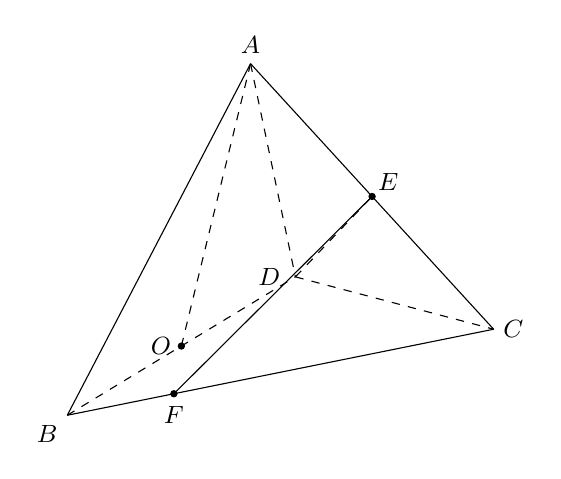
\begin{tikzpicture}[scale=0.95, font=\small]
  \coordinate (A) at (2.45,4.70);
  \coordinate (B) at (0.00,0.00);
  \coordinate (C) at (5.70,1.15);
  \coordinate (D) at (3.05,1.85);
  \coordinate (O) at (1.525,0.925);
  \coordinate (E) at (4.075,2.925);
  \coordinate (F) at (1.425,0.2875);

  % 可见棱
  \draw (A) -- (B);
  \draw (A) -- (E) -- (C);
  \draw (B) -- (F) -- (C);
  \draw (E) -- (F);
  % 隐蔽棱
  \draw[dashed] (A) -- (D);
  \draw[dashed] (A) -- (O);
  \draw[dashed] (B) -- (D);
  \draw[dashed] (D) -- (C);
  \draw[dashed] (D) -- (E);

  \fill (O) circle (1.4pt);
  \fill (E) circle (1.4pt);
  \fill (F) circle (1.4pt);
  \node[above] at (A) {$A$};
  \node[below left] at (B) {$B$};
  \node[right] at (C) {$C$};
  \node[left=2pt] at (D) {$D$};
  \node[left=1pt, inner sep=2.5pt] at (O) {$O$};
  \node[above right, inner sep=2pt] at (E) {$E$};
  \node[below=2pt, inner sep=2.5pt] at (F) {$F$};
\end{tikzpicture}
\end{center}
\nopagebreak[4]
\Needspace{4\baselineskip}
\textbf{解析}

\Needspace{5\baselineskip}
由 $CB=CD=\sqrt5$，$O$ 为 $BD$ 的中点得 $CO\perp BD$，且
\nopagebreak[4]
\[BO=OD=1,\qquad CO=\sqrt{CB^2-BO^2}=\sqrt{5-1}=2 .\]
\Needspace{5\baselineskip}
以 $O$ 为原点，$OB$ 方向为 $x$ 轴正方向，$OC$ 方向为 $y$ 轴正方向，$OA$ 方向为 $z$ 轴正方向建系（$AO\perp$ 平面 $BCD$），则
\nopagebreak[4]
\[B(-1,0,0),\quad D(1,0,0),\quad C(0,2,0),\quad A(0,0,2).\]
\Needspace{5\baselineskip}
$E$ 为 $AC$ 中点，故 $E(0,1,1)$；由 $BF=\dfrac14BC$ 得
\nopagebreak[4]
\[F=B+\frac14(C-B)=\left(-\frac34,\frac12,0\right).\]

\gksubpart{（1）}

\nopagebreak[4]
\[\overrightarrow{AB}=(-1,0,-2),\qquad \overrightarrow{DE}=E-D=(-1,1,1).\]
\Needspace{5\baselineskip}
设直线 $AB$ 与 $DE$ 所成角为 $\alpha$，则
\nopagebreak[4]
\[\cos\alpha=\frac{\left|\overrightarrow{AB}\cdot\overrightarrow{DE}\right|}{\left|\overrightarrow{AB}\right|\left|\overrightarrow{DE}\right|}
=\frac{|1+0-2|}{\sqrt5\cdot\sqrt3}=\frac1{\sqrt{15}}=\frac{\sqrt{15}}{15}.\]

\gksubpart{（2）}

\Needspace{5\baselineskip}
平面 $CDE$：$\overrightarrow{DC}=(-1,2,0)$，$\overrightarrow{DE}=(-1,1,1)$，取法向量
\nopagebreak[4]
\[\boldsymbol n_1=\overrightarrow{DC}\times\overrightarrow{DE}=(2,1,1)\]
（验证：$\boldsymbol n_1\cdot\overrightarrow{DC}=-2+2+0=0$，$\boldsymbol n_1\cdot\overrightarrow{DE}=-2+1+1=0$ ）。

\Needspace{5\baselineskip}
平面 $FDE$：$\overrightarrow{DF}=\left(-\dfrac74,\dfrac12,0\right)$，$\overrightarrow{DE}=(-1,1,1)$，
\nopagebreak[4]
\[\boldsymbol n_2=\overrightarrow{DF}\times\overrightarrow{DE}=\left(\frac12,\frac74,-\frac54\right)\ \parallel\ (2,7,-5).\]

\Needspace{5\baselineskip}
于是两平面夹角 $\theta$ 满足
\nopagebreak[4]
\[\cos\theta=\frac{\left|\boldsymbol n_1\cdot\boldsymbol n_2\right|}{\left|\boldsymbol n_1\right|\left|\boldsymbol n_2\right|}
=\frac{|4+7-5|}{\sqrt6\cdot\sqrt{4+49+25}}=\frac{6}{\sqrt6\cdot\sqrt{78}}=\frac{6}{6\sqrt{13}}=\frac1{\sqrt{13}},\]
\Needspace{5\baselineskip}
故
\nopagebreak[4]
\[\sin\theta=\sqrt{1-\frac1{13}}=\sqrt{\frac{12}{13}}=\frac{2\sqrt3}{\sqrt{13}}=\frac{2\sqrt{39}}{13}.\]

\gkanswer{答案（1）：$\dfrac{\sqrt{15}}{15}$。以 $O$ 为原点、$BD$ 为 $x$ 轴建系，$\overrightarrow{AB}=(-1,0,-2)$，$\overrightarrow{DE}=(-1,1,1)$，$|\cos\langle\overrightarrow{AB},\overrightarrow{DE}\rangle|=\dfrac1{\sqrt{15}}=\dfrac{\sqrt{15}}{15}$。}

\gkanswer{答案（2）：$\dfrac{2\sqrt{39}}{13}$。平面 $CDE$ 的法向量取 $(2,1,1)$，平面 $FDE$ 的法向量取 $(2,7,-5)$，两平面夹角余弦为 $\dfrac1{\sqrt{13}}$，故 $\sin\theta=\sqrt{1-\dfrac1{13}}=\dfrac{2\sqrt{39}}{13}$。}

\end{answer}
\begin{answer}
\gksolhead{23}{}

\textbf{题目}：

甲口袋中装有 $2$ 个黑球和 $1$ 个白球，乙口袋中装有 $3$ 个白球。现从甲、乙两口袋中各任取一个球交换放入另一口袋，重复 $n$ 次这样的操作，记甲口袋中黑球个数为 $X_n$，恰有 $2$ 个黑球的概率为 $p_n$，恰有 $1$ 个黑球的概率为 $q_n$。

（1） 求 $p_1$，$q_1$ 和 $p_2$，$q_2$；

（2） 求 $2p_n+q_n$ 与 $2p_{n-1}+q_{n-1}$ 的递推关系式和 $X_n$ 的数学期望 $E(X_n)$（用 $n$ 表示）。

\Needspace{4\baselineskip}
\textbf{解析}

每次操作后两只口袋仍各有 $3$ 个球，黑球总数为 $2$，故 $X_n\in\{0,1,2\}$，且「甲袋有 $k$ 个黑球」等价于「乙袋有 $2-k$ 个黑球」。

先写出状态转移（从甲、乙各取一球交换）：

\begin{itemize}
\item 状态 $X=2$：甲袋 $2$ 黑 $1$ 白，乙袋 $3$ 白。甲给出黑球的概率为 $\dfrac23$，此时甲黑球数变为 $1$；甲给出白球的概率为 $\dfrac13$，仍为 $2$。故
\end{itemize}
\nopagebreak[4]
\[P(2\to1)=\frac23,\qquad P(2\to2)=\frac13 .\]
\begin{itemize}
\item 状态 $X=1$：甲袋 $1$ 黑 $2$ 白，乙袋 $1$ 黑 $2$ 白。甲给出黑球：概率 $\dfrac13$，再按乙给黑（$\dfrac13$）或白（$\dfrac23$）分别为 $1$、$0$ 个黑球；甲给出白球：概率 $\dfrac23$，再按乙给黑（$\dfrac13$）或白（$\dfrac23$）分别为 $2$、$1$ 个黑球。故
\end{itemize}
\nopagebreak[4]
\[P(1\to0)=\frac13\cdot\frac23=\frac29,\quad P(1\to1)=\frac13\cdot\frac13+\frac23\cdot\frac23=\frac59,\quad P(1\to2)=\frac23\cdot\frac13=\frac29 .\]
\begin{itemize}
\item 状态 $X=0$：甲袋 $3$ 白，乙袋 $2$ 黑 $1$ 白。甲只能给出白球，乙给黑球的概率为 $\dfrac23$，故
\end{itemize}
\nopagebreak[4]
\[P(0\to1)=\frac23,\qquad P(0\to0)=\frac13 .\]

\gksubpart{（1）}

\Needspace{5\baselineskip}
初始 $p_0=1$，$q_0=0$。第一次操作后
\nopagebreak[4]
\[p_1=\frac13,\qquad q_1=\frac23 .\]
\Needspace{5\baselineskip}
第二次操作：
\nopagebreak[4]
\[p_2=p_1\cdot P(2\to2)+q_1\cdot P(1\to2)=\frac13\times\frac13+\frac23\times\frac29=\frac19+\frac4{27}=\frac7{27},\]
\nopagebreak[4]
\[q_2=p_1\cdot P(2\to1)+q_1\cdot P(1\to1)+r_1\cdot P(0\to1)=\frac13\times\frac23+\frac23\times\frac59+0=\frac29+\frac{10}{27}=\frac{16}{27},\]
其中 $r_1=P(X_1=0)=0$。检验：$p_2+q_2=\dfrac{23}{27}$，余下 $\dfrac4{27}=q_1\cdot P(1\to0)=\dfrac23\times\dfrac29$ 正是 $P(X_2=0)$ 。

\gksubpart{（2）}

\Needspace{5\baselineskip}
记 $r_n=P(X_n=0)$，则 $p_n+q_n+r_n=1$。由全概率公式
\nopagebreak[4]
\[p_n=\frac13p_{n-1}+\frac29q_{n-1},\]
\nopagebreak[4]
\[q_n=\frac23p_{n-1}+\frac59q_{n-1}+\frac23r_{n-1},\]
\nopagebreak[4]
\[r_n=\frac29q_{n-1}+\frac13r_{n-1}.\]
\Needspace{5\baselineskip}
于是
\nopagebreak[4]
\[2p_n+q_n=\left(\frac23+\frac23\right)p_{n-1}+\left(\frac49+\frac59\right)q_{n-1}+\frac23r_{n-1}
=\frac43p_{n-1}+q_{n-1}+\frac23r_{n-1}.\]
\Needspace{5\baselineskip}
代入 $r_{n-1}=1-p_{n-1}-q_{n-1}$：
\nopagebreak[4]
\[2p_n+q_n=\frac43p_{n-1}+q_{n-1}+\frac23\left(1-p_{n-1}-q_{n-1}\right)
=\frac23p_{n-1}+\frac13q_{n-1}+\frac23
=\frac13\left(2p_{n-1}+q_{n-1}\right)+\frac23 .\]
这就是所求的递推关系式。

\Needspace{5\baselineskip}
又 $X_n$ 只取 $0,1,2$，故
\nopagebreak[4]
\[E(X_n)=2p_n+q_n .\]
\Needspace{5\baselineskip}
令 $A_n=2p_n+q_n$，则 $A_n=\dfrac13A_{n-1}+\dfrac23$，即
\nopagebreak[4]
\[A_n-1=\frac13\left(A_{n-1}-1\right).\]
\Needspace{5\baselineskip}
由 $A_1=2p_1+q_1=\dfrac23+\dfrac23=\dfrac43$ 得 $A_1-1=\dfrac13$，故
\nopagebreak[4]
\[A_n-1=\frac13\cdot\left(\frac13\right)^{n-1}=\frac1{3^n},\]
\Needspace{5\baselineskip}
即
\nopagebreak[4]
\[E(X_n)=1+\frac1{3^n}.\]
检验：$n=1$ 时 $E=1+\dfrac13=\dfrac43=2\times\dfrac13+\dfrac23$ ；$n=2$ 时 $E=1+\dfrac19=\dfrac{10}9=2\times\dfrac7{27}+\dfrac{16}{27}$ 。

\gkanswer{答案（1）：$p_1=\dfrac13$，$q_1=\dfrac23$，$p_2=\dfrac7{27}$，$q_2=\dfrac{16}{27}$。第一次操作中甲给出黑球（概率 $\dfrac23$）则黑球数变为 $1$，给出白球（概率 $\dfrac13$）则仍为 $2$；第二次按状态转移逐项相加。}

\gkanswer{答案（2）：$2p_n+q_n=\dfrac13\left(2p_{n-1}+q_{n-1}\right)+\dfrac23$，$E(X_n)=1+\dfrac1{3^n}$。由状态转移得 $p_n=\dfrac13p_{n-1}+\dfrac29q_{n-1}$ 与 $q_n=\dfrac23p_{n-1}+\dfrac59q_{n-1}+\dfrac23r_{n-1}$（$r_{n-1}=1-p_{n-1}-q_{n-1}$），相加即得递推式；又 $E(X_n)=2p_n+q_n$，解递推得 $E(X_n)=1+\dfrac1{3^n}$。}

\end{answer}